\ifdefined\included
\else
\setcounter{chapter}{2} %% Numéro du chapitre précédent ;)
\dominitoc
\faketableofcontents
\fi

\chapter{Ontologenius: A long-term semantic memory}
\minitoc

\section{Design and features}

\subsection{Why an ontology?}

\subsection{Ontology formalism}

Even if we saw that the use of ontology is today a common way to represent semantic knowledge, we will recall in this subsection the composition of an ontology. For each element composing it, we will draw a formalization then give examples using the Turtle syntax. The pieces of ontologies used in the examples of this subsection are voluntarily simplified. The introduced notations will be the ones used in the rest of this thesis and the graphical representations, both in terms of color and form, will be kept as often as possible.

On the base of the definition of a Description Logic ontology presneted in \cite{fokoue_2006_summary}, we define a semantic knowledge base $\kbs$ represented as an ontology by  $\kbs = \langle \Abox, \Tbox, \Rbox \rangle$. $\Abox$, $\Tbox$, and $\Rbox$ are respectively called the Abox, Tbox, and Rbox of the ontology.

\subsubsection{The ontology Tbox}

\begin{figure}[h!]
\centering
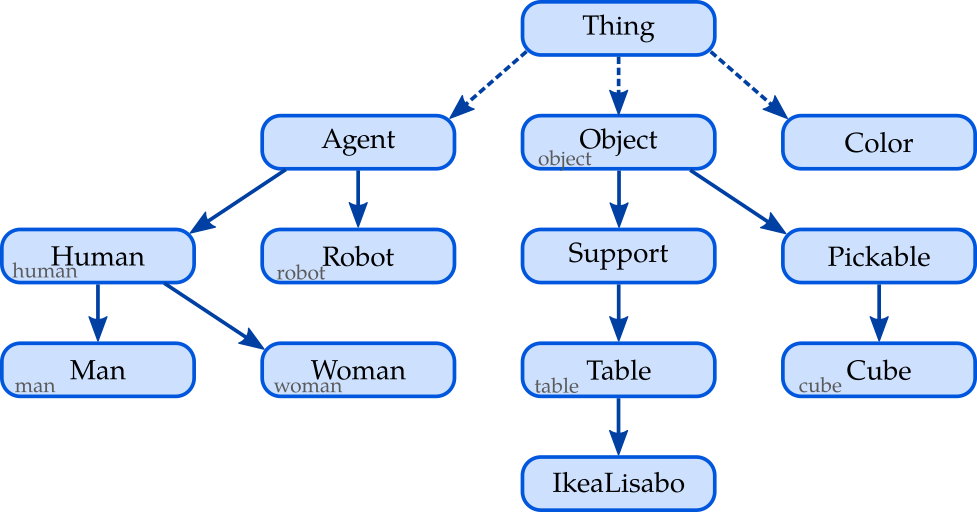
\includegraphics[scale=0.4]{figures/chapter2/Tbox.png}
\caption{\label{fig:Tbox} Representation of an ontology class hierarchy graph to illustrate the composition of a TBox. Taking the class Human, the bottom arrow has to be read as \textit{"A man is a kind of Human"}. The texts at the bottom left of the class, if there is, are the classes' labels in natural language.}
\end{figure}

The Tbox $\Tbox$ contains assertions about the \textbf{classes} (types) of the ontology. It is defined by $\Tbox = \langle \classset, H \rangle$. It can be seen as a directed acyclic graph as presented in Figure~\ref{fig:Tbox}. $\classset$ is the set of all the classes of the ontology. In our example, $\classset = \{Thing,\ Agent,\ Object, ...,\ IkeaLisabo\}$. Considering the Tbox as a graph, $H$ stores its directed edges. It represents the inheritance links between the classes (i.e. the subsumption assertions). This link is commonly referred to as the "isA" link (e.g. \textit{(Human, isA, Agent)}) and is described with the property rdfs:subClassOf in the OWL language as illustrated in the Listing~\ref{lst:Tbox}.

\begin{lstlisting}[frame=single, basicstyle=\scriptsize\ttfamily, label={lst:Tbox}, caption={Description of ontology classes in the OWL language using the Turle syntax.},captionpos=b]
:Human rdf:type owl:Class ;
       rdfs:subClassOf :Agent .

:Man   rdf:type owl:Class ;
       rdfs:subClassOf :Human .
\end{lstlisting}

\subsubsection{The ontology Rbox}

\begin{figure}[h!]
\centering
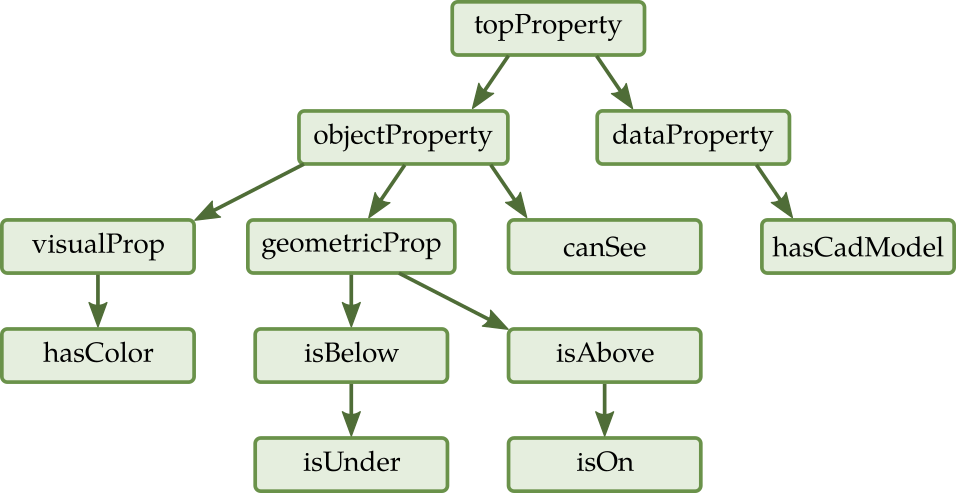
\includegraphics[scale=0.4]{figures/chapter2/Rbox.png}
\caption{\label{fig:Rbox} Representation of an ontology property hierarchy graph to illustrate the composition of an RBox. Taking the property isBelow, the bottom arrow has to be read as: \textit{"The property isUnder is a specification of the property isBelow"}.}
\end{figure}

The Rbox $\Rbox$ contains assertions about the \textbf{properties} (roles). It is at least defined by $\Rbox = \langle \propset, \inclset, \invset, \domainset, \rangeset \rangle$. In the same way as the Tbox, $\propset$ is the set of properties, and $\inclset$ stores the directed edges of the finite directed acyclic graph representing the inheritance links between the properties. Such a graph is represented in Figure~\ref{fig:Rbox}. These inheritance links aim at specifying properties. In our example, the property IsOn is a specification of the property isAbove in the way that an object being on another is an object that is above the latter and being in contact with. It is described with the property rdfs:subPropertyOf in the OWL language. 
$\invset = \{(\property, \property^{-1}) \in \propset^2\}$ is the set representing the properties inverses (\textit{e.g.} $(isOn, isUnder) \in Inv$). Describing the inverse of a property is useful first to reduce description work since if some describe a relation involving a property for which an inverse is defined, the inverse relation is also described in an underlying way. Moreover, for an algorithm exploring an ontology, knowing that a relation uses a property having an inverse can allow reducing the algorithm complexity by not considering the inverse relation into the exploration.
Finally, $\domainset$ and $\rangeset$ are two sets representing respectively the properties domains and ranges. Their are define by $\domainset = \{(\property, \class)\}$ and $\rangeset = \{(\property, \class)\}$ with $\property \in \propset$ a property and $\class \in \classset$ a class. The domain of a property informs on the type of resources that may use the property, thus the type of the subject of a triplet. The range of a property informs on the valid values applied to the property, thus the type of the object of a triplet. For the property isOn, we would therefore have $(isOn,\ Object) \in \domainset$ and $(isOn,\ Support) \in \rangeset$. In this way, we state that the property IsOn can be used to describe that an object is on top of an object being support. Domains and ranges can be used in two ways. It can be to check the consistency of an ontology by checking if the way the properties have been used corresponds to their definition. It can also be used to reason on the ontology and extract new knowledge from a given situation. If, for example, an entity is said to be on top of another that is not described as being a support, we could deduce that this second entity may be a support.

The formalization above considers only a general kind of property while the OWL language makes the distinction between two main categories. The \textbf{object properties}, linking two entities, and \textbf{data properties}, linking an entity to a value. While both are slightly different, we will only keep a general definition of a property for our formalization to simplify the future algorithm explanations. An example of the description of an object property and a data property from the Figure~\ref{fig:Rbox} are illustrated in the Listing~\ref{lst:Rbox} using the OWL language.


\begin{lstlisting}[frame=single, basicstyle=\scriptsize\ttfamily, label={lst:Rbox}, caption={Description of ontology properties in the OWL language using the Turle syntax.},captionpos=b]
:isOn  rdf:type owl:ObjectProperty ;
       rdfs:subPropertyOf :isAbove ;
       owl:inverseOf :isUnder ;
       rdfs:domain :Object ;
       rdfs:range :Support .

:hasCadModel rdf:type owl:DatatypeProperty ;
             rdfs:domain :Object .
\end{lstlisting}

\subsubsection{The ontology Abox}

\begin{figure}[h!]
\centering
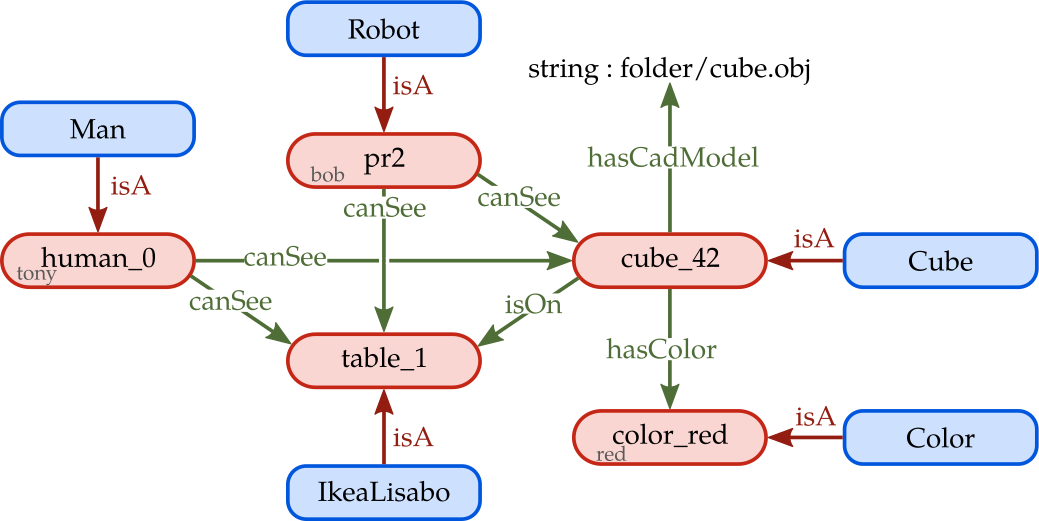
\includegraphics[scale=0.4]{figures/chapter2/Abox.png}
\caption{\label{fig:Abox}  Representation of an ontology instances graph to illustrate the composition of an ABox. Red boxes are individuals of the ontology. Green arrows are properties coming from the RBox and applied to individuals. Red arrows represent a direct inheritance link between an individual and a class coming from the TBox. The texts at the bottom left of the individuals, if there is, are the individuals' labels in natural language.}
\end{figure}

The Abox $\Abox$ contains assertions about the \textbf{entities} (individuals) of the ontology. When we refer about entities, we no more speak about general concepts but rather of instantiated concept, being either a physic or virtual entity. The Abox is defined by $\Abox = \langle \indivset, \inheritset_0, \relationset \rangle$. $\indivset$ is the set of all the entities represented in the ontology. $\inheritset_0$ the set of direct types of $\indivset$ such as $\inheritset_0 = \{(\indiv, \class) \}$ with $\indiv \in \indivset$ an individual and $\class \in \classset$ a class. In the graphical representation of an Abox in the Figure.~\ref{fig:Abox}, the red blocks are the Abox entities ($\indivset = \{human_0,\ pr2,\ ...,\ table\_1\}$) and the red arrows with the label "isA" are the intities direct types ($(cube\_42, Cube) \in \inheritset_0$).
$\relationset$ is finally the set of \textbf{relations} between entities. Such relation are in the form of triplets $(\subject, \property ,\object)$ where $\subject$ is the subject, $\property$ the property and $\object$ the object. The set of relations is thus defined by $\relationset = \{(\subject, \property ,\object) | (\subject, \object) \in \indivset^2, \property \in \propset\}$. These relations are represented by the green arrows between the entities in Figure~\ref{fig:Abox}. We can note in this figure the presence of the use of a data property "hasCadModel". This property does not link two entities, which goes against the previous definition. Regarding our formalization and to keep it tractable, we can however keep it as it is, and view the string value as an entity having for direct type a concept "String". An example of the description of an entity from the Figure~\ref{fig:Abox} is illustrated in the Listing~\ref{lst:Abox} using the OWL language.

\begin{lstlisting}[frame=single, basicstyle=\scriptsize\ttfamily, label={lst:Abox}, caption={Description of an ontology individual in the OWL language using the Turle syntax.},captionpos=b]
:cube_42  rdf:type     :Cube ;
          :hasColor    :color_red ;
          :hasCadModel "folder/cube.obj"^^string ;
          :isOn        :table_1 .
\end{lstlisting}


We just saw that in the Abox, $\inheritset_0$ contains the direct types of entities. We also saw that the classes can inherit from one each other in the Tbox, thanks to the classes inheritance directed edges stored in $H$. This means that the individuals of the Abox have inherited types. Taking the entity cube\_42 of Figure.~\ref{fig:Abox}, its direct type is the class Cube ($(cube\_42,\ Cube) \in \inheritset_0$). Regarding the Tbox represented in Figure.~\ref{fig:Tbox}, a Cube is a kind of Pickable ($(Cube,\ Pickable) \in H$), itself being a kind of Object ($(Pickable,\ Object) \in H$). We can thus say that the entity cube\_42 is a Cube, a Pickable, and an Object. To represent it, we use $\inheritset$ to denote the set of direct and inherited types. We thus have $\{ (cube\_42,\ Cube), (cube\_42,\ Pickable), (cube\_42,\ Object)\} \subset \inheritset$.

\subsubsection{Extending the ontology Tbox}

With the use of the relation set $\relationset$ of the Abox we saw that we can apply properties to individuals to link them together and form relations in the form of triplets. However, some could want to apply properties to classes to describe general links between classes. While properties domains and ranges already give such relations this can be not enough. Taking an object property hasMother, we can assign to it the class Human for domain and Woman for range. With such description, we state that a human CAN have a mother that is a woman but we do not describe that even if we do not know how it is, a human has a mother how is a woman. For this particular example, we could use cardinality constraint but we will not go as far. Taking now the data property hasCadModel of Figure~\ref{fig:Rbox}, we have applied it to a specific entity in the example of Figure~\ref{fig:Abox}. But what about a Table Lisabo (IkeaLisabo in Figure~\ref{fig:Tbox})? Any table of this model will have the same CAD model and we do not want to put this relation to every entity of this type of table. Here domains and range are not sufficient to represent it. To do so, we will use \textbf{annotation properties} applied to classes. Annotation properties are usually used to document ontologies and not to describe general relations on classes. We take thus some liberty regarding the OWL standard for convenience. However, we will try to use it in very particular cases where no other simple solution can be applied. Relations to classes using annotation properties are thus added to the definition of a Tbox $\Rbox = \langle \propset, \inclset, \invset, \domainset, \rangeset, \annotationset \rangle$, where $\annotationset$ is the set of relation between classes in the form of triplets.

\subsubsection{Elements characteristics}

In this sub-section, we have draw a formalism of an ontology in the form of $\kbs = \langle \Abox, \Tbox, \Rbox \rangle$. All the knowledge stored in $\kbs$ are sufficient to build exploration algorithm on top of it. However, to reason on ontology aditional descriptions are necessary in the form of properties characteristics. We do not add them to the knowledge base formalism but enumerate them bellow: 

\begin{itemize}
	\item \textbf{Symmetric property}: If the relation $(x, p, y)$ holds in $\relationset$ with $p$ being a symmetric property, the relation $(y, p, p)$ is also part of $\relationset$.
	\item \textbf{Asymmetric property}: If the relation $(x, p, y)$ holds in $\relationset$ with $p$ being an asymmetric property, the relation $(y, p, p)$ can no be part of $\relationset$.
	\item \textbf{Reflexive property}: A reflexive property can be used to link an individual to itself.
	\item \textbf{Irreflexive property}: An irreflexive property can not be used to link an individual to itself.
	\item \textbf{Functional property}: Every individual can be linked by a functional property to at most one other individual. By this way, if ${(x, p, y), (x, p, z)} \subset \relationset$, then $y = z$.
	\item \textbf{Inverse functional property}: Every individual can holds an iverse functional property at most one.  By this way, if ${(x, p, y), (z, p, y)} \subset \relationset$, then $x = z$.
	\item \textbf{Transitive property}: A transitive property describe a link between two individuals x and z whenever it exist a link between x and y, and y with z with this property. If ${(x, p, y), (y, p, z)} \subset \relationset$ with p a transitive property, then $(x, p, z) \in \relationset$.
	\item \textbf{Property chain axiom}: While the transitive property characteristic decsribe a link between several individuls with the same property, the chain axiom does the same with distinct properties. Given the chain $p_1 \bullet p_2 \Rightarrow p_3$, if ${(x, p_1, y), (y, p_2, z)} \subset \relationset$, then $(x, p_3, z) \in \relationset$.
	\item \textbf{Disjoinction}: Given two disjoint elements (classes or properties), a third element can not inherit of the both disjoint elements.
\end{itemize}

\subsubsection{Labeling functions}

We saw in the previous chapter that the semantic knowledge base is part of what we assimilate to be the declarative memory. The particularity of such memory is the ability to speak about the knowledge it stores. In this way, we introduce a labeling function $\labelfunc$ for any element of the ontology. This labeling function is specified for the individuals ($\alabel$), the classes ($\tlabel$), and the properties ($\plabel$). Considering the individuals labeling function $\alabel: \indivset \rightarrow Lbl$ with $Lbl$ a set of communicable names encoded as UTF8 string in our implementation. The same holds for the other two labeling functions.

\subsubsection{Ontology for Human-Robot Interaction}

Because we are working in the field of Human-Robot Interaction, it is mandatory for the robotic agent to be able to represent its own knowledge but also to represent an estimate of its human partners' knowledge. Such features will be explained later in this thesis and we only introduce the related notation for the moment.
We define the robot's own simbolic knowledge base $\kbs^R = \langle \Abox^R, \Tbox^R, \Rbox^R\rangle$.
Then, for each human agent $H_i$ the robot knows, we concider the agent's semantic knowledge $\kbs^{H_i} = \langle \Abox^{H_i}, \Tbox^{H_i}, \Rbox^{H_i} \rangle$.
The robot's global knowledge thus encompasses both its own semantic representation of the environment as well as an \textbf{estimation} of the other agent's knowledge.
In the rest of this thesis, we will simply use the notation $\kbs$ in cases where the used knowledge base does not matter.

\subsubsection{Ontology formalism recap}

The ontology definition used all along this thesis is summarized in Table~\ref{tab:onto_symboles}.

\begin{table}[h]
\caption{The list of symbols of used to define a semantic knowledge base as an ontology }
\label{tab:onto_symboles}
\begin{tabular}{ll}
{\ul \textbf{$\Abox$ ABox entities/indiv}} & {\ul \textbf{$\Tbox$ TBox classes/concepts}}  \\
$\indivset$: set of entities               & $\classset$: set of classes  \\
$\inheritset_0$: entities' direct types        & $H$: classes inheritance links \\
$\relationset$: relations between entities    & $\annotationset$: relations between classes  \\
$\alabel$: individuals labeling function & $\tlabel$: classes labeling function \\
 & \\
\multicolumn{2}{l}{{\ul \textbf{$\Rbox$ RBox roles/properties}}}                          \\
$\propset$: set of properties              &                                              \\
$\inclset$: properties inheritance links       & $\invset$: properties inverses                   \\
$\domainset$: properties' domains sets     & $\rangeset$: properties' ranges sets   \\
$\plabel$: properties labeling function & \\
\end{tabular}
\end{table}


\subsection{Desired features}


\section{Architecture}

\subsection{Permanent versus temporary data structure}

\subsection{Concepts' identifier versus name in natural language}

\subsection{Resoning to enrich the knowledge}



\section{Managing others' estimated knowledge}

\subsection{Ontologenius multi-instances principle}

\subsection{Catching knowledge at a given moment}

\subsection{Exploring several possible mental states at once}



\section{Using Ontologenius in robotic applications}

\subsection{Inserting new knowledge}

\subsection{Retrieving knowledge}

\subsubsection{Low-level queries}

\subsubsection{SPARQL-like interface}

\subsection{The Application Programming Interface}

\subsubsection{Debbuging tool}



\section{Computational preformance evaluation}

\subsection{Concepts recovery}

\subsection{Low-level queries}

\subsection{SPAQRL queries}

Lorem ipsum dolor sit amet, consectetur adipiscing elit. Sed non risus. Suspendisse lectus tortor, dignissim sit amet, adipiscing nec, ultricies sed, dolor. Cras elementum ultrices diam. Maecenas ligula massa, varius a, semper congue, euismod non, mi. Proin porttitor, orci nec nonummy molestie, enim est eleifend mi, non fermentum diam nisl sit amet erat. Duis semper. Duis arcu massa, scelerisque vitae, consequat in, pretium a, enim. Pellentesque congue. Ut in risus volutpat libero pharetra tempor. Cras vestibulum bibendum augue. Praesent egestas leo in pede. Praesent blandit odio eu enim. Pellentesque sed dui ut augue blandit sodales. Vestibulum ante ipsum primis in faucibus orci luctus et ultrices posuere cubilia Curae; Aliquam nibh. Mauris ac mauris sed pede pellentesque fermentum. Maecenas adipiscing ante non diam sodales hendrerit.

Ut velit mauris, egestas sed, gravida nec, ornare ut, mi. Aenean ut orci vel massa suscipit pulvinar. Nulla sollicitudin. Fusce varius, ligula non tempus aliquam, nunc turpis ullamcorper nibh, in tempus sapien eros vitae ligula. Pellentesque rhoncus nunc et augue. Integer id felis. Curabitur aliquet pellentesque diam. Integer quis metus vitae elit lobortis egestas. Lorem ipsum dolor sit amet, consectetuer adipiscing elit. Morbi vel erat non mauris convallis vehicula. Nulla et sapien. Integer tortor tellus, aliquam faucibus, convallis id, congue eu, quam. Mauris ullamcorper felis vitae erat. Proin feugiat, augue non elementum posuere, metus purus iaculis lectus, et tristique ligula justo vitae magna.
Aliquam convallis sollicitudin purus. Praesent aliquam, enim at fermentum mollis, ligula massa adipiscing nisl, ac euismod nibh nisl eu lectus. Fusce vulputate sem at sapien. Vivamus leo. Aliquam euismod libero eu enim. Nulla nec felis sed leo placerat imperdiet. Aenean suscipit nulla in justo. Suspendisse cursus rutrum augue. Nulla tincidunt tincidunt mi. Curabitur iaculis, lorem vel rhoncus faucibus, felis magna fermentum augue, et ultricies lacus lorem varius purus. Curabitur eu amet.

